% A simple LaTeX template for lab reports in TDT4258 Energy Efficient Computer Design
% by Yaman Umuroglu (yamanu@idi.ntnu.no)
% Feel free to customize the style as you see fit, but the chapters/sections mentioned in the
% template should be included with the appropriate content.

\documentclass[abstract=on]{scrreprt}
\usepackage[utf8]{inputenc}
\usepackage[toc,page]{appendix}


\usepackage{natbib}
\usepackage{graphicx}
\usepackage{listings}
\usepackage{float}
\usepackage{minted}
\usepackage{algorithm2e}
\usepackage{tabto}
\usemintedstyle{borland}
% Edit the meta.tex file to change title, group number and author names
% Fill in the report title, group number and student names here
\newcommand{\mytitle}{RSA encoding/decoding}
\newcommand{\mygroupnumber}{3}
\newcommand{\myauthor}{Torbjørn Viem Ness\\Marjeris Romero}

\title{\mytitle}
\author{\myauthor}
\date{\today}



\begin{document}
% The title page, edit if you want to customize it
\begin{titlepage}

\includegraphics[height=1.5cm]{images/ntnu_logo.pdf}\\[1cm]   
\begin{center}

 
% Upper part of the page
~\\[1.5cm]

\textsc{\Large TFE4141 Design of Digital Systems 1\\Laboratory Report}\\[0.5cm]

% Set the title of the Document between two horizontal lines
\hrule ~\\[0.2cm]
{\huge \bfseries \mytitle}\\[0.4cm]		% print the title of the document
\hrule ~\\[1.5cm]

% Additional Information about the document
\begin{minipage}{0.4\textwidth}
    \centering
	\large
		\emph{Group \mygroupnumber:}\\~\\
		\myauthor
\end{minipage}

\vfill

% Bottom of the page
{\large \today}

\end{center}
\end{titlepage}


% Main matter - edit corresponding file under content/ to change

\begin{abstract}
%An abstract is a short (100 to 500 words), high-level summary of the entire document. 
%For this kind of report, you would start by introducing the concept that the report talks about and the goals of the work, followed by information about how the work was done and some summary of results.
The goal for the exercise was to get implement a 128-bit RSA encryption/decryption module for a FPGA. We opted to solve this problem by using a binary add implementation for dividing the modular exponentiation in a series of squaring and multiplications. \\
For the modular multiplication operations we implemented the Montgomery multiplication algorithm. This approach is also called for the Montgomery Exponentiation method. When simulating in Vivado the implementation met the timing constraints and used little area, but there are unfortunately no results from the FPGA as we had problems getting it running.


\begin{figure}[H]
\centering
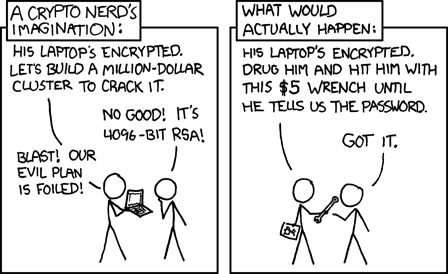
\includegraphics[width=0.7\textwidth]{images/security.png}
\caption{Mandatory XKCD: Security}
\label{fig:gamepad}
\end{figure}
\end{abstract}
\tableofcontents
\chapter{Introduction}
%Your report should start with an introduction chapter that motivates the subject in general and describes the problem you are trying to solve. 
%TODO:
The goals for the work on this term project was to give us experience with implementation of algorithms in hardware, verification by simulation, synthesis tools and to understand and evaluate other people's work by a peer-review system. \cite{ggmanual}.\cite{rsahardware}

\chapter{Background and Theory}
%This chapter should describe the theoretical background needed to understand and solve the problem. 
%For instance, a description of the hardware platform or specific components involved in this assignment, definition of concepts that are important to understand the solution should be summarized here.
%Add citations to show sources whenever appropriate, LaTeX and bibliography managers make this easy. For instance, ``I always thought something was fundamentally wrong with the universe'' \cite{adams1995hitchhiker}.
\section{Problem Description and Analysis}

- Describe the problem you are trying to solve?\\
- What are the main requirements?\\
- What do you need to investigate further before proposing a solution?\\

Design and implement hardware for an RSA encryption/decryption circuit that meets the requirements listed in figure \ref{fig:req}. The message blocks to be encrypted will be 128-bit wide, and divided into four 32-bit packets for transmission via a 32-bit wide parallell data bus into the circuit.
\begin{figure}[H]
\centering
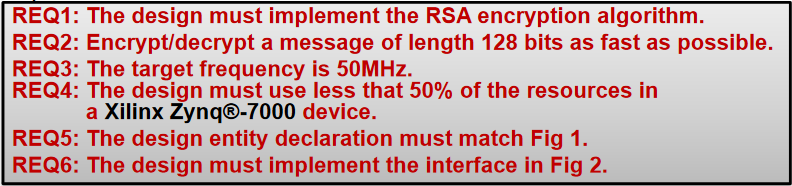
\includegraphics[width=0.7\textwidth]{images/requierements.PNG}
\caption{Design specification}
\label{fig:req}
\end{figure}
\begin{figure}[H]
\centering
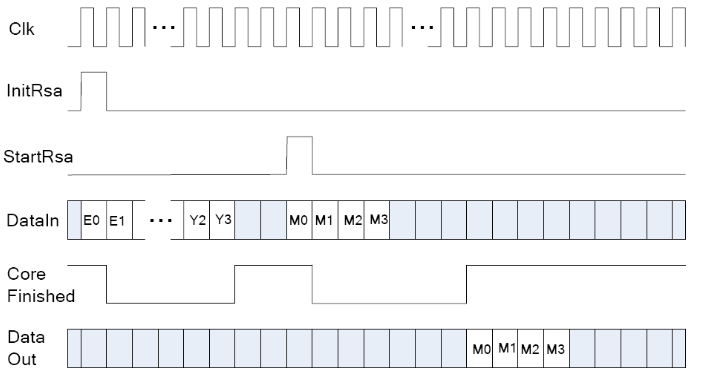
\includegraphics[width=0.7\textwidth]{images/communication.PNG}
\caption{Interface communication protocol}
\label{fig:interface}
\end{figure}
The RSA-module has to be configured with the correct keys. Each key consists of two 128-bit integers.


%%%%%%%%%%%%%%%%%%%%%%%%%%%%%%%%%%%%%%%%%%%%%%%%%%%%%%%%%%%%%%%%%%%%%%%%%
\section{RSA encryption/decryption}
RSA has its name from the creators; Ron Rivest, Adi Shamir and Len Adleman. RSA uses two different keys. One for encryption (public key); the other is for decryption (private key). \\
This is an asymmetric algorithm, with the important advantage that anyone can encrypt a message for the receiver (using the public part of the key pair), but only the receiver (who has the private key) can decrypt and read it. The method relies on a one-way function f such that it is easy to compute $Y=f(X)$, but (practically) impossible to compute $X=f_1(Y)$, unless you have the correct key $k$.

RSA is widely used in electronic commerce protocols (banking, online shopping and such), and is believed to be secure, given sufficiently long keys and the use of up-to-date implementations. As of 2016 the recommended key length is minimum 2048 bits for a good balance between speed and security.

\begin{figure}[H]
\centering
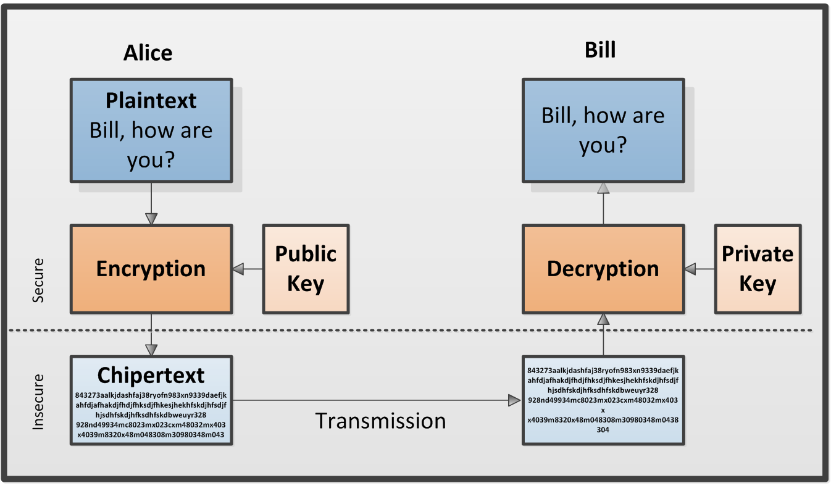
\includegraphics[width=0.7\textwidth]{images/rsa.PNG}
\caption{RSA encryption/decryption mechanism}
\label{fig:rsa}
\end{figure}

The same computation is performed for encryption and decryption, but with different parameters. The encryption and decryption keys (d,e) are related through the following equation:\\
Encryption: (public key: {e,n})
\begin{equation}
    C=M^e mod n, M<n
\end{equation}
Decryption:(private key: {d,n})
\begin{equation}
    M=C^d mod n = (M^e)^d mod n
\end{equation}

Appropriate values for e,d, and n can be found using Euler's theorem.


%%%%%%%%%%%%%%%%%%%%%%%%%%%%%%%%%%%%%%%%%%%%%%%%%%%%%%%%%%%%%%%%%%%%%%%%%%%%%%
\section{Method for computing $M^emod n$}
Modular exponentiation is achieved by replacing all multiplications in the algorithm by modular multiplications.
The computation of $M^e(mod n)$ is called modular exponentiation. In the exponentation process for the RSA algorithm, we know the exponent (e) and the modulus (n) in advance but not the base (M). 
The modular exponentiation can be broken into a series of modular multiplications and modular squaring operations.

Computing $C:= M^e (mod n)$ by first exponentiation and then performing a division to obtain the remainder $C:=(M^e)\%n $ would have resulted in an enormous space requirement. Assuming, M and e have 128 bits each, we need
\begin{equation}
    log_2(M^e)=e*log_2(M) = 2^{128}*128=2^{135} = 10^{40}
\end{equation}

The naive method of computing a modular multiplication requires e-1 modular multiplications. However not all power of M need to be computed. Using squerings you can reduce the number of multiplications. This method is called the binary method or square and multiply method.
The binary method for computing $M^emodn$ given the integers M, e, and n has two variations depending on the direction by which the bits of e are scanned: Left-to-Right(LR) and Right-to-Left(RL).

\begin{algorithm}
\setAlgoLined
    \textbf{LR Binary Method}\\
    Input: M, e, n\\
    Output: C:= M^e mod n\\
    1. if $e_{n-1}=1$ then $C:=M$ else $C:=1$\\
    2. for $i=h-2$ downto 0\\
    2a.\quad $C:=C * C (mod n)$\\
    2b.\quad if $e_{i}=1$ then $C:=C * M (mod n)$\\
    3. return $C$
\end{algorithm}

The bits of e are scanned from the most significant to the least significant, and a modular squaring is performed for each bit. A modular multiplication operation is performed only if the bit is 1.

\section{Modular Multiplication}
There are four approaches for computing P= AB (mod n).\\
Multiply and then Reduce:First multiply $t:=a*b$. Here t is a 2k-bit or 2s-word number. The reduction is accomplished by dividingt t by n, and we obtain the reminder.\\
The steps of the multiplication and reduction are interleaved (Blakley's method).\\
Brickell's method\\
Montgomery's method: This algorithm rearranges the residue class modulo n, and uses module $2^j$ arithmetic.\\

\section{Bakley's Method}
Computes $a*b mod n$ by interleaving the shift-add steps of the multiplication and the shift-substract steps of the division. This is a bit-by-bit multiplication algorithm.

\begin{algorithm}
The Blakley Algorithm\\
Input: a,b,n\\
Output: R = a * b mod n\\
1. $R:= 0$\\
2. for $i=0$ to $k-1$ \\
3. $R:=2R + a_{k-1-i}*b$\\
4. $R:= R mod n$\\
5. return $R$
\end{algorithm}

This algorithm computes the remainder R in k steps, where at each step one addition, and at most two substractions are performed.


%%%%%%%%%%%%%%%%%%%%%%%%%%%%%%%%%%%%%%%%%%%%%%%%%%%%%%%%%%%%%%%%%%%%%%%%%%%%
\section{Montgomery's Method}
Montgomery's algorithm is an efficient way of doing modular multiplication, based around the principle that... (sett inn teori fra PDF her)
This algorithm works extremly well when implemented on general-purpose computers (signal processors or microprocessors) which are capable of performing fast arithmetic modulo a power of 2. 

This algorithm replace division by n operation with division by a power of 2. This operation is easily accomplished on a computer since the numbers are represented in binary form\cite{highspeedrsa}.

The montgomery product is define as
\begin{equation}
    \bar{R}= \bar{a} * \bar{b} * r^{-1} mod n
\end{equation}
where $r^{-1}$ is the inverse of r module n
\begin{equation}
    r^{-1}*r = 1 mod n
\end{equation}
The resulting number $\bar{R}$ is the n-residue of the product
\begin{equation}
    R= a * b mod n
\end{equation}

The Montgomery algorithm computes
\begin{equation}
    MonPro(A,B) = A * B * r^{-1}mod n
\end{equation}

The product $u = A * B * 2^{-k}(mod n)$ can be compute by the following binary add-shift algorithm:
\begin{algorithm}

    1. u:=0\\
    2. for i= 0 to k-1\\
    2a.\quad u:=u + A_i * B\\
    2b.\quad if u is odd then u:=u+n\\
    2c.\quad u:=u/2\\
\end{algorithm}


%%%%%%%%%%%%%%%%%%%%%%%%%%%%%%%%%%%%%%%%%%%%%%%%%%%%%%%%%%%%%%%%%%%%%%%%%%%%%
\section{VHDL}
VHDL (\emph{Very high speed integrated circuits Hardware Description Language}) is a language used for describing and simulating/synthesizing digital logic.\\
It allows for much more efficient design of logic by formulating the desired behavior as a "program", instead of having to draw all the logic gates and connections manually.
VHDL is a hardware description language. The code describes the behavior or structure of an electronic circuit\cite{pedroni}. Its main applications include synthesis of digital cirtuits onto FPGA (Field Programmable Gate Array) or for layout/mask generation for ASIC (Application-Specific Integrated Circuit) fabrication.

VHDL allows for circuit synthesis as well as circuit simulation. Circuit synthesis translates the source code into hardware structure that implements the intended functionality, whil circuit simulation is a testing procedure to ensure correct functionality. 
\chapter{Methodology}
%This chapter should discuss the details of your implementation for the assignment. 
%Everything related to \emph{how} things were done should go here.
%Remember to avoid going into too much details, summarize appropriately and try to use figures/charts.
%Make sure you refer to the figures (such as Figure \ref{fig:universe}) and charts you add in the text.
%Avoid putting lots of source code here -- small code snippets are fine if you want to discuss something specific.
\section{Presentation of the solution}
We chose to implement the RSA circuit using one module for the MonPro operation, a datapath module with various registers for storing inputs and intermediate results and a top-level controller module with a state machine and control signals for the datapath.
In order to use Montgomery's algorithm without taking additional parameters, a simplified version of Blakley's algorithm was used to compute
\begin{equation}
    \bar{x}=1*R*mod(n), R=2^{128}
\end{equation}
\begin{equation}
    \bar{M}=M*R*mod(n), R=2^{128}
\end{equation}


\subsection{Blakley module}
In our case
The blakley module is implemented 

\subsection{Monpro module}


\subsection{Stitching everything together}

%\begin{figure}
%\centering
%\includegraphics[scale=1.7]{images/universe.jpg}
%\caption{A JPEG image of a galaxy. Use vector graphics instead if you can.}
%\label{fig:universe}
%\end{figure}
%%
%Add content in this section that describes how you tested and verified the correctness of your implementation, with respect to the requirements of the assignment.
\section{Verification plan}
- Write a verification plan.\\
- What metrics will you use to decide when you are done verifying?
(pass rate, code coverage, functional coverage).\\
- Demonstrate the use of assertions \\
- What bring up test strategy have you planned?\\ 
- Discuss/Analyze/Conclude\\
\\
Each submodule of the design was verified with its own testbench.
The RSAcore module was verified using the testbenches provided by Øystein Gjermundnes.
\\
Improvements in the verification plan would have been to use Bitvis library.
\chapter{Results}
%In this chapter, you should discuss the results you have obtained from your implementation.
%These can be correctness results, i.e whether the implementation behaved as expected, or numerical results that express runtime or energy measurements.
 
\subsection{Synthesis and test on FPGA}

- Measure area and performance

- Prove that the design actually works on FPGA

\subsection{Discussion of the results}
 
Analysis and discussion of problems, solutions and measured results is necessary in order to make the right decisions. Discussion should therefore be integrated into all parts of the report. 

- What is done, what can be improved (future work).
\chapter{Conclusion}
%This chapter should be a look back at the entire report and summarizing the problem, the solution and the obtained results.
While the project assignment wasn't entirely successful, the submodules were working and yielding output in accordance to that of the corresponding Python models.

\section{Evaluation of the Assignment}
%You can include comments about the assignment itself here. While this part is not obligatory and not graded, it is valuable feedback to the course staff that can be used to improve the exercises in the future.


% Bibliography - edit references.bib and use the \cite command in text
\bibliographystyle{plain}
\bibliography{references}
\begin{appendices}
\chapter{Modules}
\section{Python implementation}
\inputminted[
framesep=2mm,
baselinestretch=1.2,
fontsize=\footnotesize,
linenos]{python}{../Project/monexp.py}

\section{RSACore.vhd}
\inputminted[
framesep=2mm,
baselinestretch=1.2,
fontsize=\footnotesize,
linenos]{vhdl}{../Project/VHDL/RSA_module.srcs/sources_1/new/RSACore.vhd}

\section{ControlFSM.vhd}
\inputminted[
framesep=2mm,
baselinestretch=1.2,
fontsize=\footnotesize,
linenos]{vhdl}{../Project/VHDL/RSA_module.srcs/sources_1/new/ControlFSM.vhd}

\section{Datapath.vhd}
\inputminted[
framesep=2mm,
baselinestretch=1.2,
fontsize=\footnotesize,
linenos]{vhdl}{../Project/VHDL/RSA_module.srcs/sources_1/new/Datapath.vhd}

\section{MonPro.vhd}
\inputminted[
framesep=2mm,
baselinestretch=1.2,
fontsize=\footnotesize,
linenos]{vhdl}{../Project/VHDL/RSA_module.srcs/sources_1/new/monpro.vhd}

\section{Blakley.vhd}
\inputminted[
framesep=2mm,
baselinestretch=1.2,
fontsize=\footnotesize,
linenos]{vhdl}{../Project/VHDL/RSA_module.srcs/sources_1/new/blakley.vhd}

\section{Register\_enable\_reset\_n.vhd}
\label{app:register_enable_reset_n}
\inputminted[
framesep=2mm,
baselinestretch=1.2,
fontsize=\footnotesize,
linenos]{vhdl}{../Project/VHDL/RSA_module.srcs/sources_1/new/register_enable_reset_n.vhd}

\chapter{Testbenches}
\section{Blakley\_tb.vhd}
\inputminted[
framesep=2mm,
baselinestretch=1.2,
fontsize=\footnotesize,
linenos]{vhdl}{../Project/VHDL/RSA_module.srcs/sim_1/new/blakley_tb.vhd}

\section{Monpro\_tb.vhd}
\inputminted[
framesep=2mm,
baselinestretch=1.2,
fontsize=\footnotesize,
linenos]{vhdl}{../Project/VHDL/RSA_module.srcs/sources_1/new/monpro_tb.vhd}


\end{appendices}

\end{document}
